\chapter{Plan de proyecto}

En este apartado se presenta la planificación seguida a lo largo de todo el proyecto. Se especifican una serie de tareas diferenciadas entre sí que a continuación serán detalladas en profundidad.\\ Para dar por finalizada una tarea, y así poder pasar a la siguiente, ésta ha debido ser revisada previamente por el tutor. \\ Dentro del plan de estudios de la titulación, el trabajo de fin de grado tiene una carga de 12 créditos ECTS, y teniendo en cuenta que cada crédito ECTS equivale a 25 horas obtenemos, que el proyecto debe ser completado en 300 horas. De esta manera la planificación que procederemos a desarrollar en esta sección, se elabora considerando que el horario va a ser de lunes a viernes con jornadas de 3 horas de trabajo.\\

\section{Descripción de las tareas}
\subsection{Planificación del proyecto}
\label{tareaPlanificacion}
La planificación del proyecto corresponde a la primera tarea. Se subdivide el proyecto en las propias tareas que se están comentando en este punto, se realiza una estimación de tiempo de la que se genera un diagrama de Gantt que se puede consultar en la Figura \ref{fig:Gantt}, y una estimación de costos, que queda reflejada en la sección \ref{Costos}.\\

Se estima que esta tarea tendrá una duración de 5 horas.

\subsection{Estudio del algoritmo Box counting}
Con esta tarea se deja un tiempo para obtener formación sobre el algoritmo Box counting, conocer cómo funciona el \textit{"Fixed grid scan"}, y entender la implementación inicial escrita en Matlab. Para la realización de esta tarea se requiere de la adquisición de unas nociones básicas de Matlab debido al desconocimiento previo del lenguaje.\\

Se estima que esta tarea tendrá una duración de 10 horas.

\subsection{Implementación en C++ del algoritmo Box counting}
Una vez se haya comprendido el funcionamiento del algoritmo con el que se va a trabajar a lo largo de todo el proyecto, se procederá a su implementación secuencial en C++. Dentro de esta tarea, entra la comprobación de la corrección del código implementado, comprobando que es válido y funciona correctamente con datos reales de activación cerebral.\\

Se estima que esta tarea tendrá una duración de 10 horas.

\subsection{Experimentación y toma de tiempos del algoritmo sin paralelizar}
Se deja como tarea una etapa para la experimentación y toma de tiempos del algoritmo secuencial obtenido de la tarea anterior. Para la toma de tiempos se seguirá la metodología que se expone en el capítulo siguiente. El objetivo de la toma de tiempos del algoritmo secuencial es poder realizar comparaciones con las versiones que se implementen posteriormente, y medir que versión proporciona mejores aceleraciones.\\

Se estima que esta tarea tendrá una duración de 5 horas.

\subsection{Paralelización del algoritmo con OpenACC}
Se planifica una tarea que conlleva la búsqueda de bibliografía y el estudio del estándar de programación OpenACC. El objetivo de esto es poder añadir al código secuencial las directivas OpenACC necesarias para explotar el paralelismo que nos aporta el uso de una CPU multicore.\\

Se estima que esta tarea tendrá una duración de 70 horas.

\subsection{Experimentación y toma de tiempos de la paralelización con OpenACC}
Se planifica como tarea una etapa para la experimentación y toma de tiempos del código resultante de la tarea anterior. Además se analizarán los tiempos obtenidos y se compararán con los tiempos obtenidos en la etapa de experimentación del código secuencial mediante el cálculo de las aceleraciones.\\

Se estima que esta tarea tendrá una duración de 10 horas.

\subsection{Paralelización del algoritmo con CUDA}
Se planifica una tarea que conlleva la búsqueda de bibliografía y el estudio de la plataforma de programación CUDA. De esta manera, en esta fase del proyecto, se implementará todo lo necesario para aprovechar la computación de propósito general en unidades de procesamiento gráfico (GPGPU) para aprovechar las tarjetas gráficas de la compañía Nvidia.\\

La paralelización con CUDA es un poco más compleja que la paralelización con OpenACC, por tanto, para realizar esta tarea se empezará implementado la versión en 2D, y partiendo de esa versión como base, se desarrollarán la versión 3D y 4D.\\

Se estima que esta tarea tendrá una duración de 110 horas.

\subsection{Experimentación y toma de tiempos de la paralelización con CUDA}
Se deja como tarea una etapa para la experimentación y toma de tiempos del código resultante de la tarea anterior. Además se analizarán los tiempos obtenidos y se compararán con los tiempos obtenidos en la etapa de experimentación del código secuencial y con la etapa de experimentación del código paralelizado con OpenACC mediante el cálculo de las aceleraciones.\\

Se estima que esta tarea tendrá una duración de 20 horas.

\subsection{Análisis de los resultados obtenidos}
El objetivo de esta tarea, es dejar un tiempo para la comparación de todos los resultados obtenidos en las etapas de experimentación y toma de tiempos, así como discusión y redacción de conclusiones sobre los resultados obtenidos.\\

Se estima que esta tarea tendrá una duración de 20 horas.

\subsection{Elaboración de la memoria}
Durante el desarrollo de todo el proyecto se irá elaborando una memoria a modo de documentación del trabajo realizado, aunque se estiman 30 horas adicionales para terminarla.

\subsection{Preparación de la defensa ante el tribunal}
Tras la entrega del trabajo, se deja un tiempo para la elaboración del material necesario para la defensa y exposición del proyecto ante el tribubal.\\

Se estima que esta tarea tendrá una duración de 10 horas.


\section{Diagrama de Gantt}
Como anticipábamos en \textit{"\nameref{tareaPlanificacion}"}, la primera etapa del proyecto es la planificación temporal del mismo. Para ello el primer paso es la división del proyecto en tareas y su correspondiente especificación. A continuación, se realiza una estimación de los días necesarios que tomará cada tarea, teniendo en cuenta que se trabajará en jornadas de 3 horas diarias de lunes a viernes. Finalmente, se hace una planificación temporal de todas las tareas en base a la estimación de tiempo realizada, obteniendo así el diagrama de la Figura \ref{fig:Gantt}. En la tabla \ref{fig:Planificacion} se puede consultar la estimación de cada tarea así como, su fecha de inicio y finalización\\ Debido a la falta de experiencia en un proyecto de este tipo, esta especificación puede que no sea suficientemente detallada, en los siguientes capítulos se profundizará más en la descripción de las distintas tareas.\\ Esto es una planificación inicial del proyecto, como en todo proyecto es posible que surjan inconvenientes que retrasen alguna de las tareas o que se hayan subestimado alguna de ellas.
\newpage
\begin{figure}[h]
    \raggedleft
    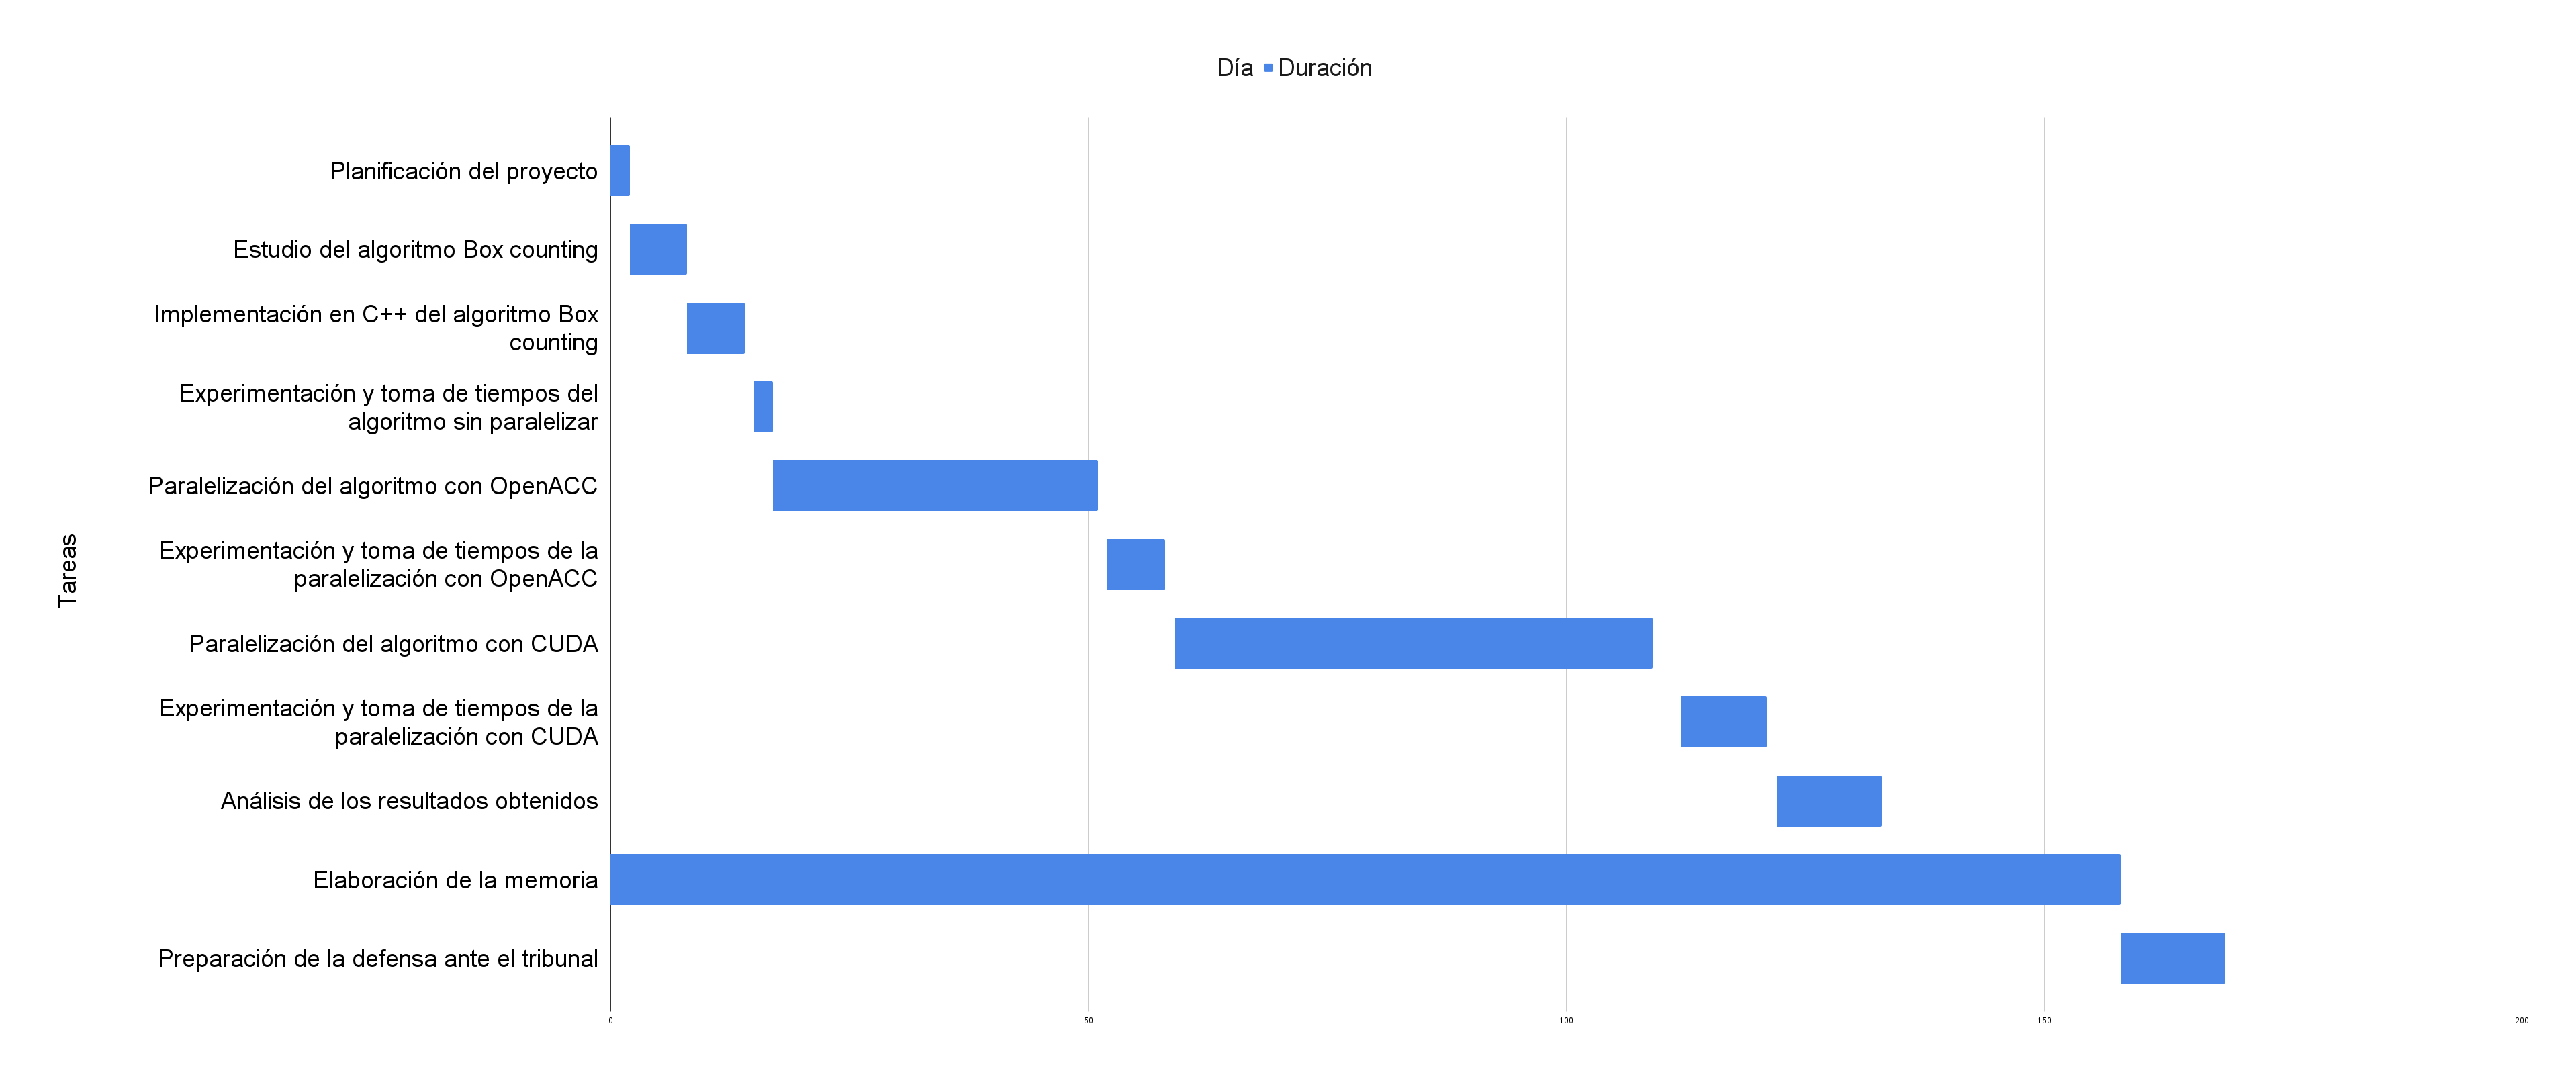
\includegraphics[scale=0.145]{img/Diagrama de Gantt2.png}
    \caption{Diagrama de Gantt}
    \label{fig:Gantt}
\end{figure}

\begin{table}[H]
    \centering
    \begin{adjustbox}{max height=\textheight, max width=\textwidth}
    \begin{tabular}{|clllrrl|} 
    \hline
    \rowcolor{black} \multicolumn{1}{|l}{}  & \textcolor{white}{Tareas} & \textcolor{white}{Fecha de inicio}         & \textcolor{white}{Fecha de finalización} & \textcolor{white}{Horas estimadas}&\\                                      
    \hline
    \rowcolor{white} \multicolumn{1}{|l}{}  & \textcolor{black}{Planificación del proyecto} & \textcolor{black}{1/2/2021}         & \textcolor{black}{3/2/2021} & \textcolor{black}{5}&\\
    \hline
    \rowcolor{white} \multicolumn{1}{|l}{}  & \textcolor{black}{Estudio del algoritmo Box counting} & \textcolor{black}{3/2/2021}         & \textcolor{black}{9/2/2021} & \textcolor{black}{10}&\\  
    \hline
    \rowcolor{white} \multicolumn{1}{|l}{}  & \textcolor{black}{Implementación en C++ del algoritmo Box counting} & \textcolor{black}{9/2/2021}         & \textcolor{black}{15/2/2021} & \textcolor{black}{10}\\
    \hline
    \rowcolor{white} \multicolumn{1}{|l}{}  & \textcolor{black}{Experimentación y toma de tiempos del algoritmo sin paralelizar} & \textcolor{black}{16/2/2021}         & \textcolor{black}{18/2/2021} &\textcolor{black}{5}&\\
    \hline
    \rowcolor{white} \multicolumn{1}{|l}{}  & \textcolor{black}{Paralelización del algoritmo con OpenACC} & \textcolor{black}{18/2/2021}         & \textcolor{black}{24/3/2021} &\textcolor{black}{70}\\
    \hline
    \rowcolor{white} \multicolumn{1}{|l}{}  & \textcolor{black}{Experimentación y toma de tiempos de la paralelización con OpenACC} & \textcolor{black}{25/3/2021}         & \textcolor{black}{31/3/2021} &\textcolor{black}{10}\\
    \hline
    \rowcolor{white} \multicolumn{1}{|l}{}  & \textcolor{black}{Paralelización del algoritmo con CUDA} & \textcolor{black}{1/4/2021}         & \textcolor{black}{21/5/2021} &\textcolor{black}{110}\\
    \hline
    \rowcolor{white} \multicolumn{1}{|l}{}  & \textcolor{black}{Experimentación y toma de tiempos de la paralelización con CUDA} & \textcolor{black}{24/5/2021}         & \textcolor{black}{2/6/2021} &\textcolor{black}{20}\\
    \hline
    \rowcolor{white} \multicolumn{1}{|l}{}  & \textcolor{black}{Análisis de los resultados obtenidos} & \textcolor{black}{3/6/2021}         & \textcolor{black}{14/6/2021} &\textcolor{black}{20}&\\
    \hline
    \rowcolor{white} \multicolumn{1}{|l}{}  & \textcolor{black}{Elaboración de la memoria} & \textcolor{black}{1/2/2021}         & \textcolor{black}{9/7/2021} &\textcolor{black}{30}&\\
    \hline
    \rowcolor{white} \multicolumn{1}{|l}{}  & \textcolor{black}{Preparación de la defensa ante el tribubal} & \textcolor{black}{9/7/2021}         & \textcolor{black}{20/7/2021} &\textcolor{black}{10}&\\                                  
    \hline
    \end{tabular}
    \end{adjustbox}
    \caption{Planificación temporal de las tareas}
    \label{fig:Planificacion}
\end{table}

\section{Recursos}
\subsection{Recursos Humanos}
Para la realización del proyecto se cuenta con Miguel Ángel Posadas Arráez como autor del mismo, y con el Profesor Dr. Juan Ruiz de Miras como tutor encargado de la supervisión del mismo.

\subsection{Recursos Software}
\label{RecursosSoftware}
Debido a que este proyecto corresponde al ámbito académico, se presta especial atención en utilizar herramientas con licencia libre, o que sean accesibles mediante la adquisición de algún tipo de licencia de estudiante, beneficiandonos así, de las ventajas que nos proporciona pertenecer a la Universidad de Granada.\\

\begin{itemize}
    \item Como alternativa a Matlab, se utiliza Octave. \cite{unknown-author-2021B}.
    \item Como herramienta de control de versiones, se utiliza GitHub, siendo posible obtener una licencia de estudiante en la siguiente referencia \cite{unknown-author-2021}.
    \item Para la elaboración de hojas de cálculo y generación de gráficos, se utiliza la suite ofimática de Google, accediendo siempre con la cuenta corporativa de la Universidad de Granada (dominio go.ugr.es).
    \item Para la elaboración de la memoria LaTeX como procesador de textos. \cite{unknown-author-no-dateD}.
    \item Para la paralelización mediante el uso de tarjeta gráfica, se utiliza el CUDA Toolkit, \cite{unknown-author-no-date}.
    \item Para la paralelización mediante el uso de los mútliples núcleos de la CPU, se utiliza OpenACC. \cite{unknown-author-no-dateB}.
    \item El sistema operativo del equipo principal utilizado para el desarrollo del proyecto es Ubuntu 20.04.2 LTS. \cite{unknown-author-no-dateE}.
\end{itemize}

\subsection{Recursos Hardware}
\label{RecursosHardware}
Para el desarrollo del proyecto se utilizan dos equipos, un ordenador portatil y un servidor. En la tabla \ref{fig:Hardware} quedan reflejadas las características más importantes de los distintos equipos.

\begin{table}[H]
    \centering
    \begin{adjustbox}{max height=\textheight,max width=\textwidth}
    \begin{tabular}{|clllrrl|} 
    \hline
    \rowcolor{black} \multicolumn{1}{|l}{}   & \textcolor{white}{Plataforma}         & \textcolor{white}{} \\  
    \hline
    \rowcolor{white} \multicolumn{1}{|l}{Plataforma}   & \textcolor{black}{PC}         & \textcolor{black}{Servidor} \\  
    \hline
    \rowcolor{white} \multicolumn{1}{|l}{Sistema Operativo}    & \textcolor{black}{Ubuntu 20.04 LTS $x86-64$}         & \textcolor{black}{Debian Linux 5.8.10-1 $x86-64$}        \\                                                            
    \hline
    \midrule
    \hline
    \rowcolor{black} \multicolumn{1}{|l}{}   & \textcolor{white}{CPU}         & \textcolor{white}{} \\  
    \hline
    \rowcolor{white} \multicolumn{1}{|l}{Model}    & \textcolor{black}{Intel(R) Core(TM) i7-7700HQ CPU @ 2.80GHz}         & \textcolor{black}{2 x Intel(R) Xeon(R) Silver 4210 CPU @ 2.20GHz}        \\ 
    \hline
    \rowcolor{white} \multicolumn{1}{|l}{Cores-thread}    & \textcolor{black}{4-8}         & \textcolor{black}{20-40}        \\  
    \hline
    \rowcolor{white} \multicolumn{1}{|l}{RAM}    & \textcolor{black}{12 GB}         & \textcolor{black}{96 GB}        \\ 
    \hline
    \rowcolor{black} \multicolumn{1}{|l}{}   & \textcolor{white}{GPU}         & \textcolor{white}{} \\  
    \hline                          
    \rowcolor{white} \multicolumn{1}{|l}{Model}    & \textcolor{black}{GeForce GTX 1050 Mobile}         & \textcolor{black}{GeForce RTX 3090}        \\ 
    \hline
    \rowcolor{white} \multicolumn{1}{|l}{Computing Capability}   & \textcolor{black}{6.1}         & \textcolor{black}{8.0} \\  
    \hline
    \rowcolor{white} \multicolumn{1}{|l}{Arquitectura}   & \textcolor{black}{Pascal}         & \textcolor{black}{Ampere} \\  
    \hline 
    \rowcolor{white} \multicolumn{1}{|l}{MPs}   & \textcolor{black}{5}         & \textcolor{black}{82} \\  
    \hline 
    \rowcolor{white} \multicolumn{1}{|l}{SPs}   & \textcolor{black}{640}         & \textcolor{black}{10496} \\  
    \hline  
    \rowcolor{white} \multicolumn{1}{|l}{Memoria Global}   & \textcolor{black}{2 GB}         & \textcolor{black}{24 GB} \\  
    \hline  
    \rowcolor{white} \multicolumn{1}{|l}{Tamaño de Warp}   & \textcolor{black}{32}         & \textcolor{black}{32} \\  
    \hline  
    \rowcolor{white} \multicolumn{1}{|l}{Nº Máximo de hebras por bloque}   & \textcolor{black}{1024}         & \textcolor{black}{1024} \\  
    \hline  
    \rowcolor{white} \multicolumn{1}{|l}{Nº Máximo de hebras por SMP}   & \textcolor{black}{2048}         & \textcolor{black}{1536} \\  
    \hline  
    \rowcolor{white} \multicolumn{1}{|l}{Tamaño de caché L2}   & \textcolor{black}{524288 B}         & \textcolor{black}{6291456 B} \\  
    \hline  
    \rowcolor{white} \multicolumn{1}{|l}{Memoria compartida por bloque}   & \textcolor{black}{49152 B}         & \textcolor{black}{49152 B} \\  
    \hline  
    \rowcolor{white} \multicolumn{1}{|l}{Registros por bloque}   & \textcolor{black}{65536}         & \textcolor{black}{65536} \\  
    \hline  
    \rowcolor{white} \multicolumn{1}{|l}{ECC}   & \textcolor{black}{Desactivado}         & \textcolor{black}{Desactivado} \\  
    \hline  
    \rowcolor{white} \multicolumn{1}{|l}{Consumo energético}   & \textcolor{black}{75 W}         & \textcolor{black}{350 W} \\  
    \hline    
    \end{tabular}
    \end{adjustbox}
    \caption{Tabla comparativa de las plataformas hardware y software utilizadas para las medidas de tiempos}
    \label{fig:Hardware}
\end{table}



El primer equipo (Identificado como PC en la Tabla \ref{fig:Hardware}) tuvo un coste inicial de 1100€, basándonos en \cite{unknown-author-no-dateG}, tiene un periodo de amortización de 6 años, luego cada año tiene un coste de 183.33€. Como este proyecto está enmarcado en un cuatrimestre, se estima que el coste de amortización del equipo es de 45.83€.\\

El servidor tiene un precio de 24000€, se establece un periodo de amortización de 6 años basándonos de nuevo en \cite{unknown-author-no-dateG}. Obtenemos que el del servidor tiene un costo de 4000€/año, que resulta en 11€/día. Como se han requerido 7 días del servidor, concluimos que el costo total por este recurso ha sido de 77€.\\ 

\subsection{Organización del personal}
Dentro del plan de estudios de la titulación \cite{unknown-author-no-dateC}, el Trabajo de Fin de Grado (TFG), tiene una carga de 12 créditos ECTS. Sabiendo que cada crédito ECTS equivale a 25 horas, el proyecto debe ser planificado en un total de 300 horas.\\


\subsection{Estimación de costos del proyecto}
\label{Costos}

Como ya se ha comentado previamente, el proyecto debe ser planificado en 300 horas, por tanto en este apartado se va a realizar un desglose de los gastos que conlleva el proyecto, especificando a que se dedicará cada hora. Para el cálculo del presupuesto se va a tomar como salario promedio 8.22 €/hora según lo especificado en \cite{unknown-author-2021C}.\\ En la Tabla \ref{fig:CosteTareas} se puede consultar el desglose de los gastos de cada tarea.

\begin{table}[H]
    \centering
    \begin{adjustbox}{max height=\textheight,max width=\textwidth}
    \begin{tabular}{|clllrrl|} 
    \hline
    \rowcolor{black} \multicolumn{1}{|l}{}  & \textcolor{white}{Tareas} & \textcolor{white}{Duración (h)}         & \textcolor{white}{Importe (€)} \\                                      
    \hline
    \rowcolor{white} \multicolumn{1}{|l}{}  & \textcolor{black}{Planificación del proyecto} & \textcolor{black}{5 h}         & \textcolor{black}{41.1€} &\\
    \hline
    \rowcolor{white} \multicolumn{1}{|l}{}  & \textcolor{black}{Estudio del algoritmo Box counting} & \textcolor{black}{10 h}         & \textcolor{black}{82.2€} &\\  
    \hline
    \rowcolor{white} \multicolumn{1}{|l}{}  & \textcolor{black}{Implementación en C++ del algoritmo Box counting} & \textcolor{black}{10 h}         & \textcolor{black}{82.2€} \\
    \hline
    \rowcolor{white} \multicolumn{1}{|l}{}  & \textcolor{black}{Experimentación y toma de tiempos del algoritmo sin paralelizar} & \textcolor{black}{5 h}         & \textcolor{black}{41.1€}&\\
    \hline
    \rowcolor{white} \multicolumn{1}{|l}{}  & \textcolor{black}{Paralelización del algoritmo con OpenACC} & \textcolor{black}{70 h}         & \textcolor{black}{575.4€} &\\
    \hline
    \rowcolor{white} \multicolumn{1}{|l}{}  & \textcolor{black}{Experimentación y toma de tiempos de la paralelización con OpenACC} & \textcolor{black}{10 h}         & \textcolor{black}{82.2€} &\\
    \hline
    \rowcolor{white} \multicolumn{1}{|l}{}  & \textcolor{black}{Paralelización del algoritmo con CUDA} & \textcolor{black}{110 h}         & \textcolor{black}{904.2€} \\
    \hline
    \rowcolor{white} \multicolumn{1}{|l}{}  & \textcolor{black}{Experimentación y toma de tiempos de la paralelización con CUDA} & \textcolor{black}{20 h}         & \textcolor{black}{164.4€} &\\
    \hline
    \rowcolor{white} \multicolumn{1}{|l}{}  & \textcolor{black}{Análisis de los resultados obtenidos} & \textcolor{black}{20 h}         & \textcolor{black}{164.4€} &\\
    \hline
    \rowcolor{white} \multicolumn{1}{|l}{}  & \textcolor{black}{Elaboración de la memoria} & \textcolor{black}{30 h}  &\textcolor{black}{246.6€}&\\
    \hline
    \rowcolor{white} \multicolumn{1}{|l}{}  & \textcolor{black}{Preparación de la defensa ante el tribubal} & \textcolor{black}{10 h}         & \textcolor{black}{82.2€} &\\                                  
    \hline
    \rowcolor{white} \multicolumn{1}{|l}{}  & \textcolor{black}{Total} & \textcolor{black}{300h}         & \textcolor{black}{2466€} &\\                                  
    \hline
    \end{tabular}
    \end{adjustbox}
    \caption{Desglose de costes de las tareas}
    \label{fig:CosteTareas}
\end{table}

En la Tabla \ref{fig:CosteRecursos} se especifican todos los recursos necesarios para la realización del proyecto con su coste asociado.

\begin{table}[H]
    \centering
    \begin{adjustbox}{max height=\textheight, max width=\textwidth}
    \begin{tabular}{|clllrrl|} 
    \hline
    \rowcolor{black} \multicolumn{1}{|l}{}  & \textcolor{white}{Recursos} & \textcolor{white}{Importe (€)}         & \textcolor{white}{Detalle} \\                                      
    \hline
    \rowcolor{white} \multicolumn{1}{|l}{}  & \textcolor{black}{Recursos Humanos} & \textcolor{black}{2466€ €}         & \textcolor{black}{Total obtenido en la Tabla \ref{fig:CosteTareas}} &\\
    \hline
    \rowcolor{white} \multicolumn{1}{|l}{}  & \textcolor{black}{Conexión a Internet} & \textcolor{black}{90 €}         & \textcolor{black}{6 meses desde febrero hasta julio a un precio de 15€/mes } &\\
    \hline
    \rowcolor{white} \multicolumn{1}{|l}{}  & \textcolor{black}{Recursos Software} & \textcolor{black}{0 €}         & \textcolor{black}{Ver \textit{\nameref{RecursosSoftware}}} &\\
    \hline
    \rowcolor{white} \multicolumn{1}{|l}{}  & \textcolor{black}{Amortización del equipo personal} & \textcolor{black}{45.83 €}         & \textcolor{black}{Coste de amortización del equipo detallado en \textit{\nameref{RecursosHardware}}} &\\
    \hline
    \rowcolor{white} \multicolumn{1}{|l}{}  & \textcolor{black}{Amortización del servidor} & \textcolor{black}{77 €}         & \textcolor{black}{Coste de amortización del servidor detallado en \textit{\nameref{RecursosHardware}}} &\\
    \hline
    \rowcolor{white} \multicolumn{1}{|l}{}  & \textcolor{black}{Total} & \textcolor{black}{2678.83 €}         & \textcolor{black}{} &\\
    \hline
    \end{tabular}
    \end{adjustbox}
    \caption{Desglose de costes de los recursos}
    \label{fig:CosteRecursos}
\end{table}
